%%%%%%%%%%%%%%%%%%%%%%%%%%%%%%%%%%%%%%%%%
% Dreuw & Deselaer's Poster
% LaTeX Template
% Version 1.0 (11/04/13)
%
% Created by:
% Philippe Dreuw and Thomas Deselaers
% http://www-i6.informatik.rwth-aachen.de/~dreuw/latexbeamerposter.php
%
% This template has been downloaded from:
% http://www.LaTeXTemplates.com
%
% License:
% CC BY-NC-SA 3.0 (http://creativecommons.org/licenses/by-nc-sa/3.0/)
%
%%%%%%%%%%%%%%%%%%%%%%%%%%%%%%%%%%%%%%%%%

%----------------------------------------------------------------------------------------
%	PACKAGES AND OTHER DOCUMENT CONFIGURATIONS
%----------------------------------------------------------------------------------------

\documentclass[final,hyperref={pdfpagelabels=false}]{beamer}

\usepackage[orientation=portrait,size=a1,scale=1.4]{beamerposter} % Use the beamerposter package for laying out the poster with a portrait orientation and an a0 paper size

\usetheme{I6pd2} % Use the I6pd2 theme supplied with this template

\usepackage[english]{babel} % English language/hyphenation
\usepackage[utf8]{inputenc} % Required for inputting international characters
%\usepackage[T1]{fontenc}
\usepackage{algorithm}
\usepackage[noend]{algpseudocode}
\usepackage{hyperref}

\usepackage{amssymb}
\usepackage{amsmath}
\usepackage{wrapfig}


\usepackage{amsmath,amsthm,amssymb,latexsym,physics} % For including math equations, theorems, symbols, etc

%\usepackage{times}\usefonttheme{professionalfonts}  % Uncomment to use Times as the main font
%\usefonttheme[onlymath]{serif} % Uncomment to use a Serif font within math environments

\boldmath % Use bold for everything within the math environment

\usepackage{booktabs} % Top and bottom rules for tables

\graphicspath{{figures/}} % Location of the graphics files

\usecaptiontemplate{\small\structure{\insertcaptionname~\insertcaptionnumber: }\insertcaption} % A fix for figure numbering

%----------------------------------------------------------------------------------------
%	TITLE SECTION
%----------------------------------------------------------------------------------------

\title{\huge Sistema de Transcrição Melódica em Tempo Real} % Poster title
\bigskip

\author{Autor: Alessandro Wagner Palmeira \\ Supervisor: Prof. Dr. Marcelo Gomes de Queiroz} % Author(s)

\institute{Instituto de Matemática e Estatística - Universidade de São Paulo} % Institution(s)

%----------------------------------------------------------------------------------------
%	FOOTER TEXT
%----------------------------------------------------------------------------------------

\newcommand{\leftfoot}{\url{https://linux.ime.usp.br/~rulojuka/mac0499}} % Left footer text

\newcommand{\rightfoot}{\url{https://github.com/rulojuka/}} % Right footer text

%----------------------------------------------------------------------------------------

\def\changemargin#1#2{\list{}{\rightmargin#2\leftmargin#1}\item[]}
\let\endchangemargin=\endlist

\addto\captionsenglish{\renewcommand{\figurename}{Figura}}

\begin{document}

\addtobeamertemplate{block end}{}{\vspace*{2ex}} % White space under blocks

\begin{frame}[t] % The whole poster is enclosed in one beamer frame

\begin{columns}[t] % The whole poster consists of two major columns, each of which can be subdivided further with another \begin{columns} block - the [t] argument aligns each column's content to the top

\begin{column}{.02\textwidth}\end{column} % Empty spacer column

\begin{column}{.465\textwidth} % The first column

%----------------------------------------------------------------------------------------
%   INTRODUCTION
%----------------------------------------------------------------------------------------

\begin{block}{Introdução}

\begin{itemize}
\item O avanço da tecnologia de Computação Musical vem trazendo novas áreas de interesse tanto acadêmicas quanto comerciais em sistemas de transcrição musical com novas técnicas de transcrição monofônicas e polifônicas, sistemas de geração automática de partituras, ressíntese, busca de informação musical e outras. Exemplos comerciais incluem jogos como Guitar Hero e Rock Band, serviços como Shazam e ScoreCloud, e aplicativos como PitchScope e intelliScore Ensemble.

\item Apesar do grande interesse acadêmico e comercial, a quantidade de software livre nessa àrea é insignificante e esse trabalho pretende prover uma implementação livre, de uso irrestrito e gratuito com uma qualidade de transcrição monofônica comparável aos softwares comerciais existentes.

Assim, nesse trabalho, pretendemos estender o trabalho de conclusão de curso de Adriano Mitre [1][2] para alcançar maior robustez, eficiência e a implementação de algumas técnicas novas.
\end{itemize}

\end{block}

%----------------------------------------------------------------------------------------
%	OBJECTIVES
%----------------------------------------------------------------------------------------

\begin{block}{Objetivos}

\begin{enumerate}
\item Transcrição em tempo real de melodias monofônicas com alto nível de robustez e eficiência
\item Implementação de técnicas novas
\item Implementação de uma interface gráfica para melhor interação com o usuário
\end{enumerate}

\end{block}

%----------------------------------------------------------------------------------------
%	Fourier
%----------------------------------------------------------------------------------------

\begin{block}{Transformada de Fourier}

A \emph{Transformada de Fourier} é o passo mais básico para muitos dos algoritmos de transcrição melódica. Ela decompõe uma função periódica em suas senóides constituintes (\emph{parciais}), como pode ser visto na figura 1.
%\newline

\begin{figure}%[!htb]
\centering
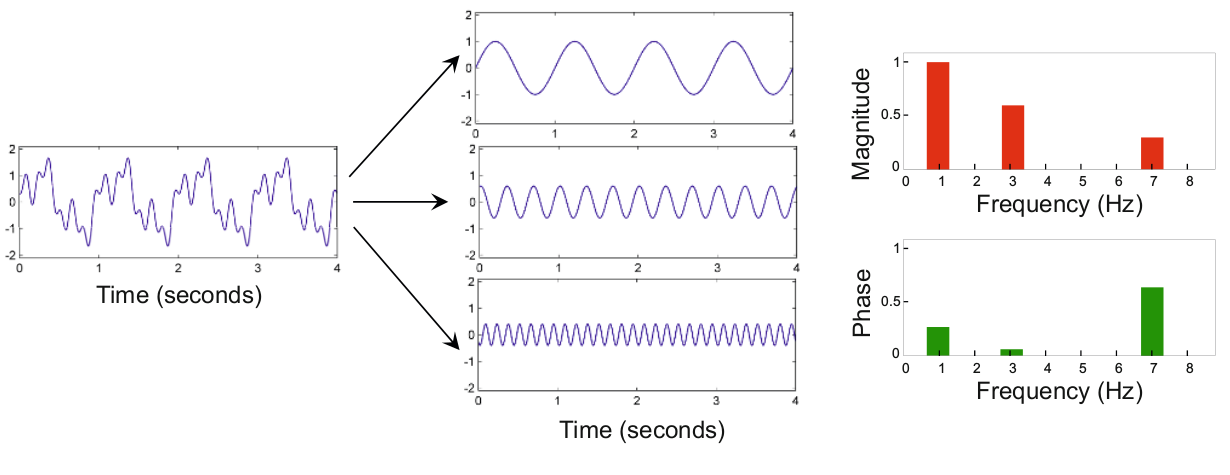
\includegraphics[width=0.7\linewidth]{fourier3}
\caption{Decomposição de um sinal em três parciais.}
\end{figure}

Se dividirmos o nosso sinal temporal em \emph{janelas} de tempo com $N$ amostras obtidas a partir de uma taxa amostral $R$, podemos utilizar um algoritmo de Transformada Discreta de Fourier para conseguir uma matriz onde cada coluna representa a Transformada de Fourier de uma dessas janelas e cada linha representa um \emph{escaninho} de $R/N$ Hz. Se escolhermos uma janela de $N=2^k$ amostras, podemos utilizar o algoritmo de Transformada Rápida de Fourier, cujo tempo de execução é $O(N\log{}N)$.
%\newline

\begin{figure}%[!htb]
\centering
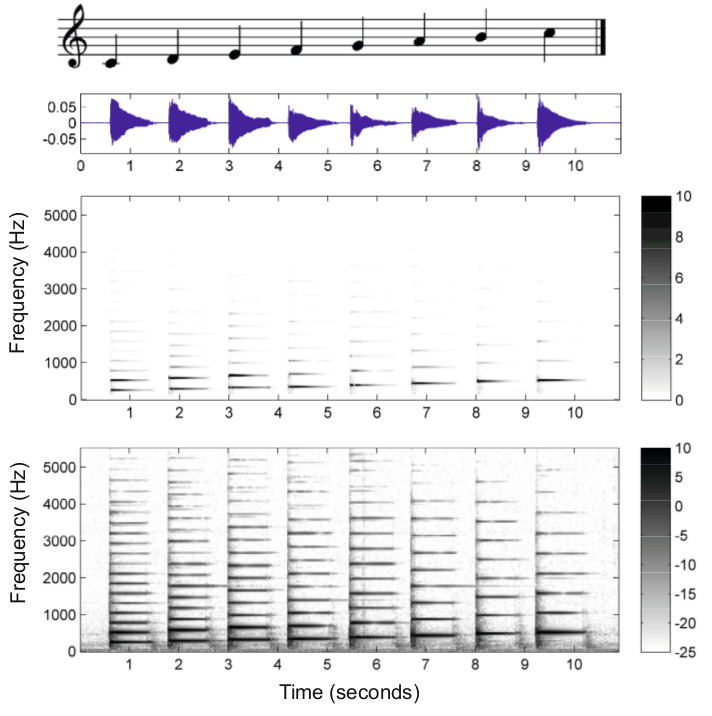
\includegraphics[width=0.7\linewidth]{fourier}
\caption{Transformada de Fourier em um sinal de áudio obtido a partir de um piano.}
\end{figure}

\end{block}

%----------------------------------------------------------------------------------------

\end{column} % End of the first column

\begin{column}{.03\textwidth}\end{column} % Empty spacer column

\begin{column}{.465\textwidth} % The second column
%----------------------------------------------------------------------------------------
\begin{block}{Transcrição em tempo real}

A detecção da \emph{Frequência Fundamental (F0)} ou transcrição melódica é um problema bastante pesquisado e comumente considerado ``resolvido'' no caso de vozes ou instrumentos monofônicos gravados.[3] Porém a questão do tempo real adiciona algumas dificuldades ao problema. Geralmente esses são os requerimentos para os algoritmos em tempo real:

\begin{changemargin}{2cm}{2cm}
\begin{itemize}
\item Capacidade de funcionar em tempo real
\item Mínimo atraso de saída (latência)
\item Acurácia na presença de ruído
\item Sensibilidade à performance musical
\end{itemize}
\end{changemargin}

Nesse contexto, apresentamos os seguintes algoritmos a serem implementados no \emph{ASyMuT - Automatic System for Music Transcription}:

\begin{changemargin}{2cm}{2cm}
     \begin{itemize}
\item \emph{Harmonic Product Spectrum} (apresentado na próxima seção)
\item \emph{Maximum Likelihood}
\item \emph{Cepstrum-Biased Harmonic Product Spectrum}
\item \emph{Weighted Autocorrelation Function}
\end{itemize}
\end{changemargin}

\end{block}

%----------------------------------------------------------------------------------------
% HPS
%----------------------------------------------------------------------------------------

\begin{block}{Harmonic Product Spectrum}
Esse algoritmo busca por uma frequência cujo produto da magnitude dos primeiros $K$ harmônicos é máximo, calculando a seguinte função para cada frequência: $$Y(\omega) = \prod _{k=1}^{K} \abs{X(\omega k))}$$
E então buscando seu máximo: $\widehat{Y} = \max\limits_{\omega_i}\{Y(\omega_i)\}$
%\newline

     \begin{figure}%[!htb]
\centering
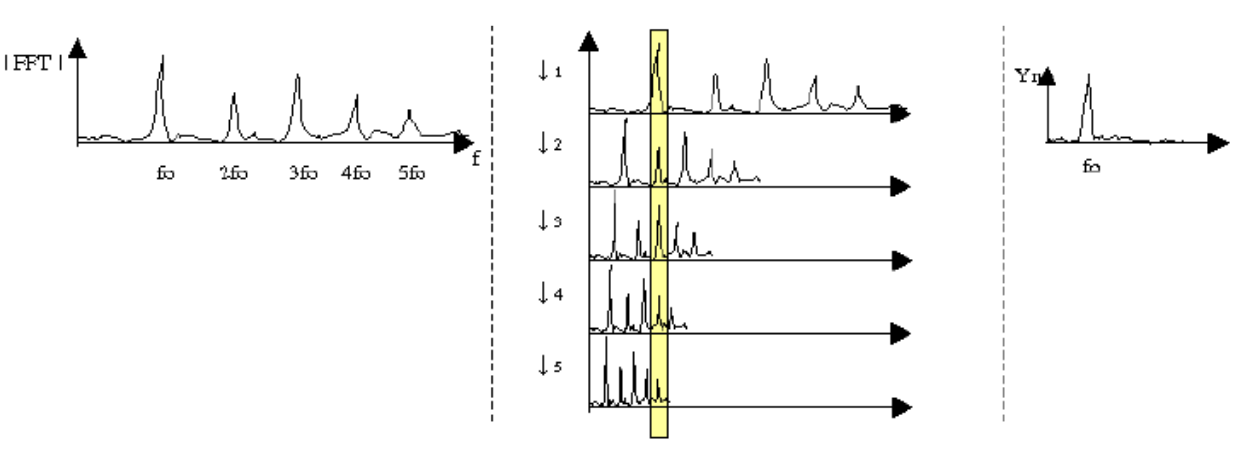
\includegraphics[width=0.85\linewidth]{hps2.png}
\caption{Harmonic Product Spectrum para $K=5$}
\end{figure}

\end{block}

%----------------------------------------------------------------------------------------
% Interface Gráfica
%----------------------------------------------------------------------------------------

\begin{block}{Interface Gráfica}

Um protótipo de interface gráfica foi implementado utilizando o arcabouço LÖVE e a linguagem Lua. A cada nota recebida do ASyMuT uma nova linha é desenhada na tela, mostrando a informação de altura de um modo visual para o músico no formato piano-roll.

Neste formato, cada linha horizontal no gráfico representa um semitom e, quanto mais para cima está o desenho da linha, mais aguda é a nota transcrita.
\begin{figure}%[!htb]
    \centering
    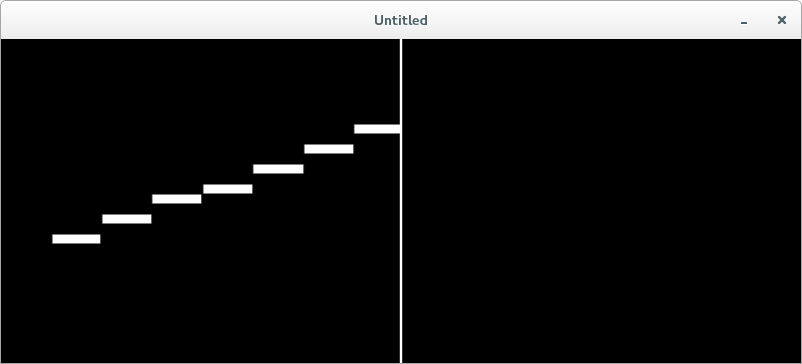
\includegraphics[width=0.6\linewidth]{screen2.png}
    \caption{Interface gráfica mostrando o piano-roll de uma escala de dó maior.}
    \end{figure}



\end{block}

%----------------------------------------------------------------------------------------
%	Referências
%----------------------------------------------------------------------------------------

\setbeamercolor{block title}{fg=black,bg=orange!70} % Change the block title color
\begin{block}{Referências}

\begin{enumerate}
\item Mitre, Adriano, and Marcelo Queiroz. ``Um sistema automático de transcrição melódica.'' Simpósio Brasileiro de Computação Musical 10 (2005): 174-185.

\item \url{https://github.com/adrianomitre/asymut}

\item De La Cuadra, Patricio, Aaron Master, and Craig Sapp.``Efficient pitch detection techniques for interactive music.'' Proceedings of the 2001 international computer music conference. 2001.
\end{enumerate}

\end{block}

%----------------------------------------------------------------------------------------

\end{column} % End of the second column

\begin{column}{.015\textwidth}\end{column} % Empty spacer column

\end{columns} % End of all the columns in the poster

\end{frame} % End of the enclosing frame

\end{document}
